\begin{refsection}

\chapter{U--Th--(Sm)--He}\label{ch:UThHe-R}

\noindent\begin{minipage}[t]{.15\linewidth}
\strut\vspace*{-\baselineskip}\newline
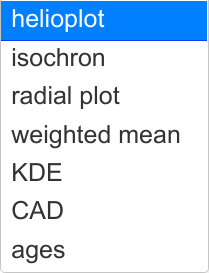
\includegraphics[width=\linewidth]{../figures/UThHePlotDevices.png}\\
\end{minipage}
\begin{minipage}[t]{.85\textwidth}
  U--Th--(Sm)--He data are provided as flat tables with eight data
  columns (Section~\ref{ch:UThHe}), in which the last two columns may
  be empty if Sm has not been measured. They can be visualised on all
  the generic plot devices, plus the helioplot.
\end{minipage}

Note that, unlike all the other methods that were discussed before, it
is not necessary to specify the \texttt{format} argument when using
the \texttt{read.data()} function. \texttt{IsoplotR} automatically
figures out whether a dataset contains Sm or not:

\begin{script}
UThHe <- read.data('UThHe.csv',method='U-Th-He')
UThSmHe <- read.data('UThSmHe.csv',method='U-Th-He')
\end{script}

\noindent which returns a simple, eight-column table.\\

\noindent\begin{minipage}[t]{.65\linewidth}
\strut\vspace*{-\baselineskip}\newline
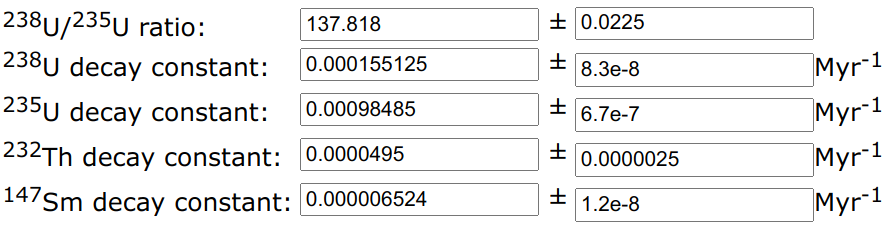
\includegraphics[width=\linewidth]{../figures/UThSmHeLambda.png}
\end{minipage}
\begin{minipage}[t]{.35\textwidth}
  The default U, Th and Sm decay constants are those proposed by
  \citet{jaffey1971}, \citet{leroux1963} and \citet{villa2020}
  respectively.
\end{minipage}

\begin{script}
# change the Sm decay constant to the Lugmair and Marti (1978) value:
settings('lambda','Sm147',0.000006540,0.000000049)
\end{script}

\section{Helioplots}\label{sec:helioplot-R}

\texttt{IsoplotR}'s \texttt{helioplot} function represents a pair of
two plotting devices that visualise U--Th--He data as a compositional
data system (Section~\ref{sec:UThHeCompositional}).\\

\noindent\begin{minipage}[t]{.18\linewidth}
\strut\vspace*{-\baselineskip}\newline

\includegraphics[width=\linewidth]{../figures/UThHelioplotLogratio.png}
\end{minipage}
\begin{minipage}[t]{.82\textwidth}
  The compositional nature of the U--Th--He system can either be
  expressed as a logratio plot or a ternary diagram
  (Figure~\ref{fig:UThHeIsochronHelioplot}).\\
\end{minipage}

\begin{script}
par(mfrow=c(1,2)) # set up a two-panel plot
helioplot(UThHe,logratio=TRUE)  # ternary diagram
helioplot(UThHe,logratio=FALSE) # logratio plot
\end{script}

\printbibliography[heading=subbibliography]

\end{refsection}
